\documentclass[a4paper,10pt]{jsarticle}

% レイアウト
\setlength{\textwidth}{\fullwidth}
\setlength{\textheight}{39\baselineskip}
\addtolength{\textheight}{\topskip}
\setlength{\voffset}{-0.5in}
\setlength{\headsep}{0.3in}
\pagestyle{myheadings}

% パッケージ
\usepackage[dvipdfmx]{graphicx}
\usepackage{amsmath,amssymb,epsfig}
\usepackage{bm}
\usepackage{ascmac}
\usepackage{pifont}
\usepackage{multirow}
\usepackage{enumerate}
\usepackage{cases}
\usepackage{type1cm}
\usepackage{cancel}
\usepackage{url}
\usepackage[dvipdfmx]{color}
\usepackage{listings,jlisting}
% 大きな中括弧
\usepackage{cases}

% 定義
\DeclareMathOperator*{\argmin}{arg\,min}
\DeclareMathOperator*{\argmax}{arg\,max}
\def\vec#1{\mbox{\boldmath$#1$}}
\def\R{{\Bbb R}}

% カウンタの設定
\setcounter{section}{0}
\setcounter{subsection}{0}
\setcounter{subsubsection}{0}
\setcounter{equation}{0}

% キャプションの図をFigに変更
\renewcommand{\figurename}{Fig.}
\renewcommand{\tablename}{Tab.}

% 式番号を式(章番号.番号)に
% \makeatletter
% \renewcommand{\theequation}{\arabic{section}.\arabic{equation}}
% \@addtoreset{equation}{section}
% \makeatother

% プログラムに色をつける
\usepackage{color}

\definecolor{codegreen}{rgb}{0,0.6,0}
\definecolor{codegray}{rgb}{0.5,0.5,0.5}
\definecolor{codepurple}{rgb}{0.58,0,0.82}
\definecolor{backcolour}{rgb}{0.95,0.95,0.92}

\lstdefinestyle{mystyle}{
    backgroundcolor=\color{backcolour},
    commentstyle=\color{codegreen},
    keywordstyle=\color{magenta},
    numberstyle=\tiny\color{codegray},
    stringstyle=\color{codepurple},
    basicstyle=\footnotesize,
    breakatwhitespace=false,
    breaklines=true,
    captionpos=b,
    keepspaces=true,
    numbers=left,
    numbersep=5pt,
    showspaces=false,
    showstringspaces=false,
    showtabs=false,
    tabsize=2
}

\lstset{style=mystyle}

% % ドキュメントの開始
\begin{document}

\section{実行方法}
\subsection{動作環境}
LinuxのディストリビューションのひとつであるUbuntuで動作を確認している.
Ubuntuで動作させるための必要なアプリケーションは以下の通りである.

\begin{lstlisting}[basicstyle=\ttfamily\footnotesize, language=Bash, frame=single, firstnumber=1, numbers=left, breaklines=true]
sudo apt-get install build-essential
sudo apt-get install cmake
sudo apt-get install gnuplot
sudo apt-get install meshlab
\end{lstlisting}

コンパイル時に必要なビルドシステムはbuild-essentialとcmakeが必要である.
そして各関節の座標系とアームの姿勢を確認するためにgnuplotを用いており,またアームのstlのデータ確認のためmeshlabというアプリケーションを用いている.

Visual Studioでのコンパイルも可能であるが,その場合Struct.hの最初の記述を変更する.

\begin{lstlisting}[basicstyle=\ttfamily\footnotesize, language=C, frame=single, firstnumber=4, numbers=left, breaklines=true]
#define _CRT_SECURE_NO_DEPRECATE
#include <stdio.h>
#include <stdlib.h>
#define _USE_MATH_DEFINES
#include <math.h>
\end{lstlisting}

\subsection{ファイル構造}
このzipの中のファイル構造を示す.

\begin{lstlisting}[basicstyle=\ttfamily\footnotesize, language=Bash, frame=single, firstnumber=1, numbers=left, breaklines=true]
.
├── CMakeLists.txt
├── Struct.h
├── document
│  └── document.pdf
├── kadai.h
├── kadai1A.cpp
├── kadai1A.h
├── kadai2A.cpp
├── kadai2A.h
├── kadai2B.cpp
├── kadai2B.h
├── main.cpp
└── plot
    ├── Arm.stl
    ├── arm.dat
    ├── plot.plt
    ├── tetra_point.dat
    ├── x.dat
    ├── y.dat
    └── z.dat
\end{lstlisting}

tetra\_point.datが三角柱を作成するための初期位置が記されたデータであり,Arm.stlが課題3の結果である.
その他のデータはgnuplotで姿勢を確認するために生成されたファイルであり,プログラムを実行すると生成される.
このデータの可視化方法を下に示す.

\begin{lstlisting}[basicstyle=\ttfamily\footnotesize, language=Bash, frame=single, firstnumber=1, numbers=left, breaklines=true]
cd plot
gnuplot
load "plot.plt"
\end{lstlisting}

\subsection{コンパイル方法と実行方法}

\begin{lstlisting}[basicstyle=\ttfamily\footnotesize, language=Bash, frame=single, firstnumber=1, numbers=left, breaklines=true]
mkdir build
cd build
cmake ..
make
./実行ファイル名
\end{lstlisting}

\section{実装した関数の説明}

\begin{lstlisting}[basicstyle=\ttfamily\footnotesize, language=C, frame=single, numbers=none, breaklines=true]
void ForwardKinematics(double joint[], double link[]);
\end{lstlisting}

\begin{itemize}
 \item ロボットアームの順運動学計算(各関節角度とリンクのパラメータ指定)
 \item 具体的な計算は次の節で示す
\end{itemize}

\begin{lstlisting}[basicstyle=\ttfamily\footnotesize, language=C, frame=single, numbers=none, breaklines=true]
void ShowTfAxis(double joint[], double link[])
\end{lstlisting}

\begin{itemize}
 \item ロボットの各軸の座標を求める
 \item 各軸での座標系を作成
 \item 外部ファイルに保存
\end{itemize}

\begin{lstlisting}[basicstyle=\ttfamily\footnotesize, language=C, frame=single, numbers=none, breaklines=true]
void ArmOutputdat(double P[][VEC_SIZE]);
\end{lstlisting}

\begin{itemize}
 \item 求めたロボットの各軸の座標を用いてリンク自体の骨格モデルを出力
\end{itemize}

\begin{lstlisting}[basicstyle=\ttfamily\footnotesize, language=C, frame=single, numbers=none, breaklines=true]
void TfAxisOutputdat(double P[][VEC_SIZE], FILE *fpx, FILE *fpy, FILE *fpz);
\end{lstlisting}

\begin{itemize}
 \item 各軸での座標系を可視化するためのファイル作成補助
\end{itemize}

\begin{lstlisting}[basicstyle=\ttfamily\footnotesize, language=C, frame=single, numbers=none, breaklines=true]
void OutputPlt();
\end{lstlisting}

\begin{itemize}
 \item リンクのモデルを出力
 \item Gnuplotで可視化
\end{itemize}

\begin{lstlisting}[basicstyle=\ttfamily\footnotesize, language=C, frame=single, numbers=none, breaklines=true]
void OutputSTL(double part1[][VEC_SIZE], double part2[][VEC_SIZE], double part3[][VEC_SIZE]);
\end{lstlisting}

\begin{itemize}
 \item 各リンクのパーツをSTL形式で出力
\end{itemize}

\begin{lstlisting}[basicstyle=\ttfamily\footnotesize, language=C, frame=single, numbers=none, breaklines=true]
void LinkCreator(double joint[], double link[]);
\end{lstlisting}

\begin{itemize}
 \item 与えられた関節角度とリンク長からアームの姿勢を求め、STLで出力
\end{itemize}

\begin{lstlisting}[basicstyle=\ttfamily\footnotesize, language=C, frame=single, numbers=none, breaklines=true]
void set_arm(double Origin[][VEC_SIZE], double P[][VEC_SIZE], double h);
\end{lstlisting}

\begin{itemize}
 \item リンクの初期姿勢を定義
 \item STLを作成するための姿勢を準備
\end{itemize}

\section{計算方法}
基準座標系$(X_0,\ Y_0,\ Z_0)$におけるハンド座標系$(X_5,\ Y_5,\ Z_5)$を求める式を示す.ただし以下に示す行列は並進移動と回転移動を同時に行っている.1リンク目から順に変換行列を示すと

\begin{eqnarray}
\label{eq:a}
  T_0 &=&
  \left[
    \begin{array}{cccc}
      \cos{\theta_1} & -\sin{\theta_1} & 0 & 0 \\
      \sin{\theta_1} & \cos{\theta_1} & 0 & 0\\
      0 & 0 & 1 & a\\
      0 & 0 & 0 & 1\\
    \end{array}
  \right]\\
  T_1 &=&
  \left[
    \begin{array}{cccc}
      1 & 0 & 0 & 0 \\
      0 & \cos{\theta_2} & -\sin{\theta_2} & 0\\
      0 & \sin{\theta_2} & \cos{\theta_2} & b\\
      0 & 0 & 0 & 1\\
    \end{array}
  \right]\\
  T_2 &=&
  \left[
    \begin{array}{cccc}
      \cos{\theta_3} & 0 & \sin{\theta_3} & 0 \\
      0 & 1 & 0 & c\\
      \sin{\theta_3} & 0 & \cos{\theta_3} & 0\\
      0 & 0 & 0 & 1\\
    \end{array}
  \right]\\
  T_3 &=&
  \left[
    \begin{array}{cccc}
      1 & 0 & 0 & 0 \\
      0 & \cos{\theta_4} & -\sin{\theta_4} & 0\\
      0 & \sin{\theta_4} & \cos{\theta_4} & d\\
      0 & 0 & 0 & 1\\
    \end{array}
  \right]\\
  T_4 &=&
  \left[
    \begin{array}{cccc}
      \cos{\theta_5} & 0 & \sin{\theta_5} & 0 \\
      0 & 1 & 0 & e\\
      \sin{\theta_5} & 0 & \cos{\theta_5} & 0\\
      0 & 0 & 0 & 1\\
    \end{array}
  \right]\\
  T_5 &=&
  \left[
    \begin{array}{cccc}
      1 & 0 & 0 & 0 \\
      0 & 1 & 0 & f\\
      0 & 0 & 1 & 0\\
      0 & 0 & 0 & 1\\
    \end{array}
  \right]
\end{eqnarray}

変換行列中に含まれている$a$,$b$,$c$,$d$,$e$,$f$は$L_1 = a+b$,$L_3 = c+d$,$L_5 = e+f$が成り立ち,リンクと同じ方向軸で回転するリンクの位置を任意の場所にできるようプログラム上ではそれぞれの別のリンクと考え変数としている.
式\eqref{eq:a}によって基準座標系$(X_0,\ Y_0,\ Z_0)$における点$P_0$からハンドの先端の座標$P_5$を求めると以下の式で表される.

\begin{equation}
\label{eq:b}
  P_5 = T_0T_1T_2T_3T_4T_5 P_0
\end{equation}

\section{結果}
それぞれの課題で結果を示す.
\subsection{課題1}
課題1は上の節で式を示した.

\subsection{課題2}
課題2はgnuplotを用いて各関節の角度を指定したときのロボットアームの姿勢と各軸での座標系を表示することで確認を行った.
この結果をFig.~\ref{fig:ロボットの姿勢と途中の関節の動作を表す座標系}に示す.Fig.~\ref{fig:ロボットの姿勢と途中の関節の動作を表す座標系}は課題3で指定された関節角度を指定した.

\begin{figure}[b]
  \centering
  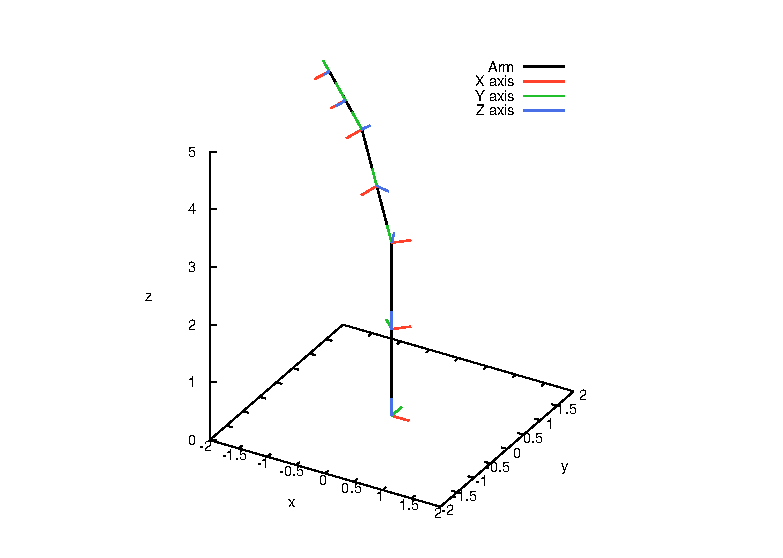
\includegraphics[width=140mm]{fig/eps/tf.eps}
  \caption{ロボットの姿勢と途中の関節の動作を表す座標系}
  \label{fig:ロボットの姿勢と途中の関節の動作を表す座標系}
\end{figure}

\subsection{課題3}
指定された角度にしたときのロボットアームの姿勢をSTLに出力したときの図をFig.~\ref{fig:ロボットアームの姿勢1}から{fig:ロボットアームの姿勢4}に示す.

\begin{figure}[b]
 \begin{minipage}{0.5\hsize}
  \begin{center}
   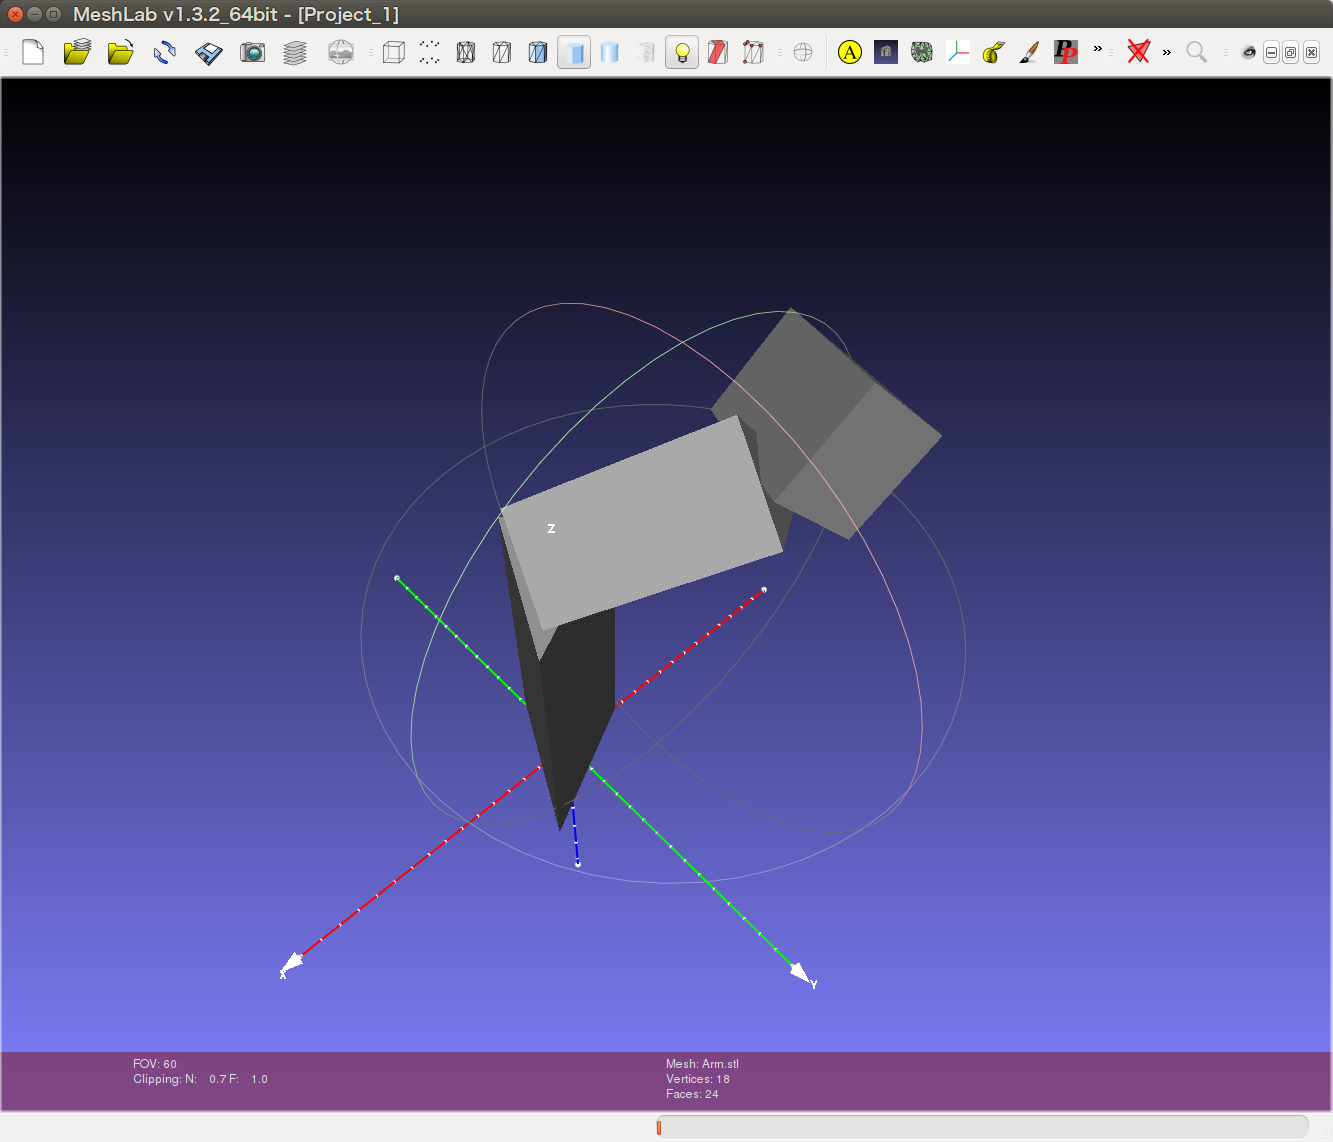
\includegraphics[width=70mm, bb = 0 0 1333 1142]{fig/png/arm1.png}
  \end{center}
  \caption{ロボットアームの姿勢1}
  \label{fig:ロボットアームの姿勢1}
 \end{minipage}
 \begin{minipage}{0.5\hsize}
  \begin{center}
   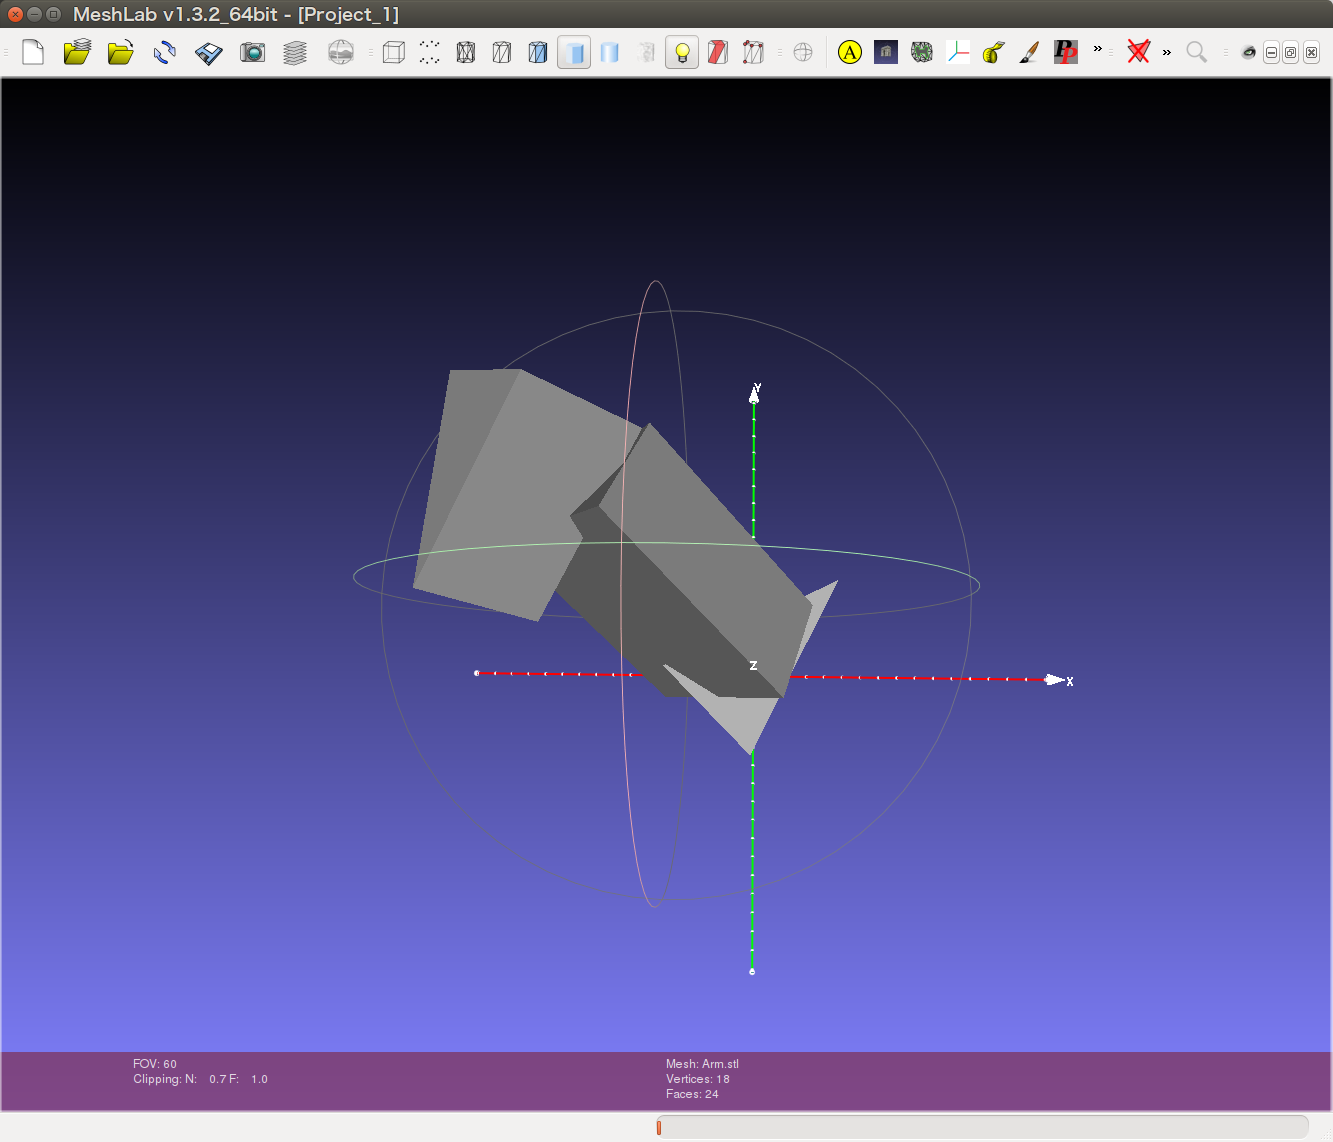
\includegraphics[width=70mm, bb = 0 0 1333 1142]{fig/png/arm2.png}
  \end{center}
  \caption{ロボットアームの姿勢2}
  \label{fig:ロボットアームの姿勢2}
 \end{minipage}
\end{figure}

\begin{figure}[b]
 \begin{minipage}{0.5\hsize}
  \begin{center}
   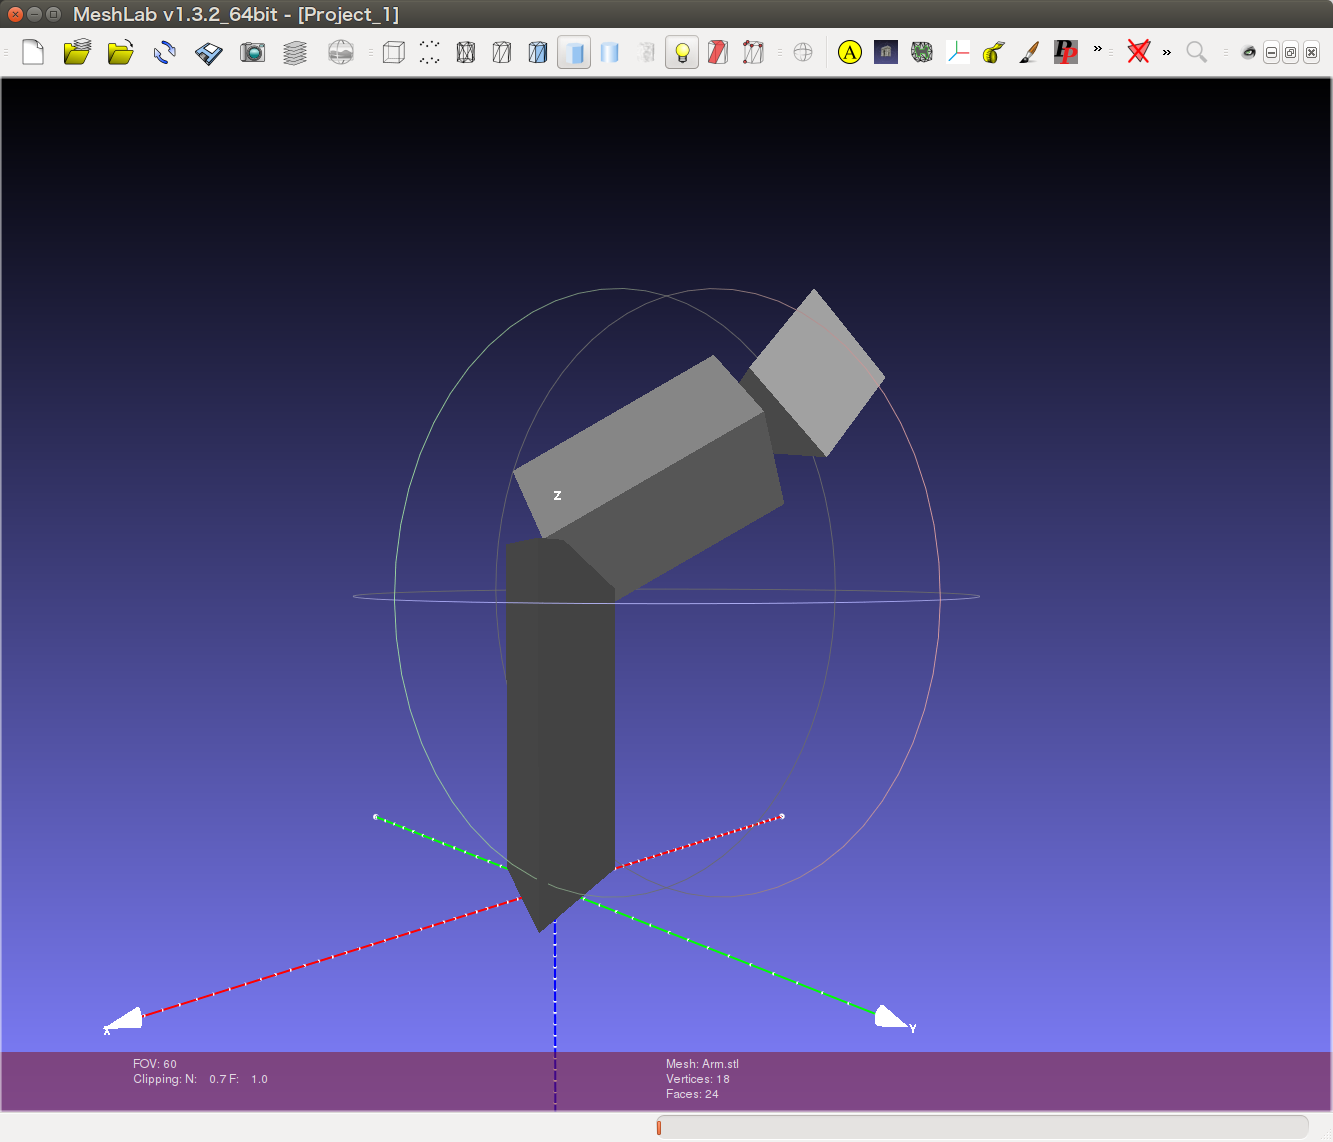
\includegraphics[width=70mm, bb = 0 0 1333 1142]{fig/png/arm3.png}
  \end{center}
  \caption{ロボットアームの姿勢3}
  \label{fig:ロボットアームの姿勢3}
 \end{minipage}
 \begin{minipage}{0.5\hsize}
  \begin{center}
   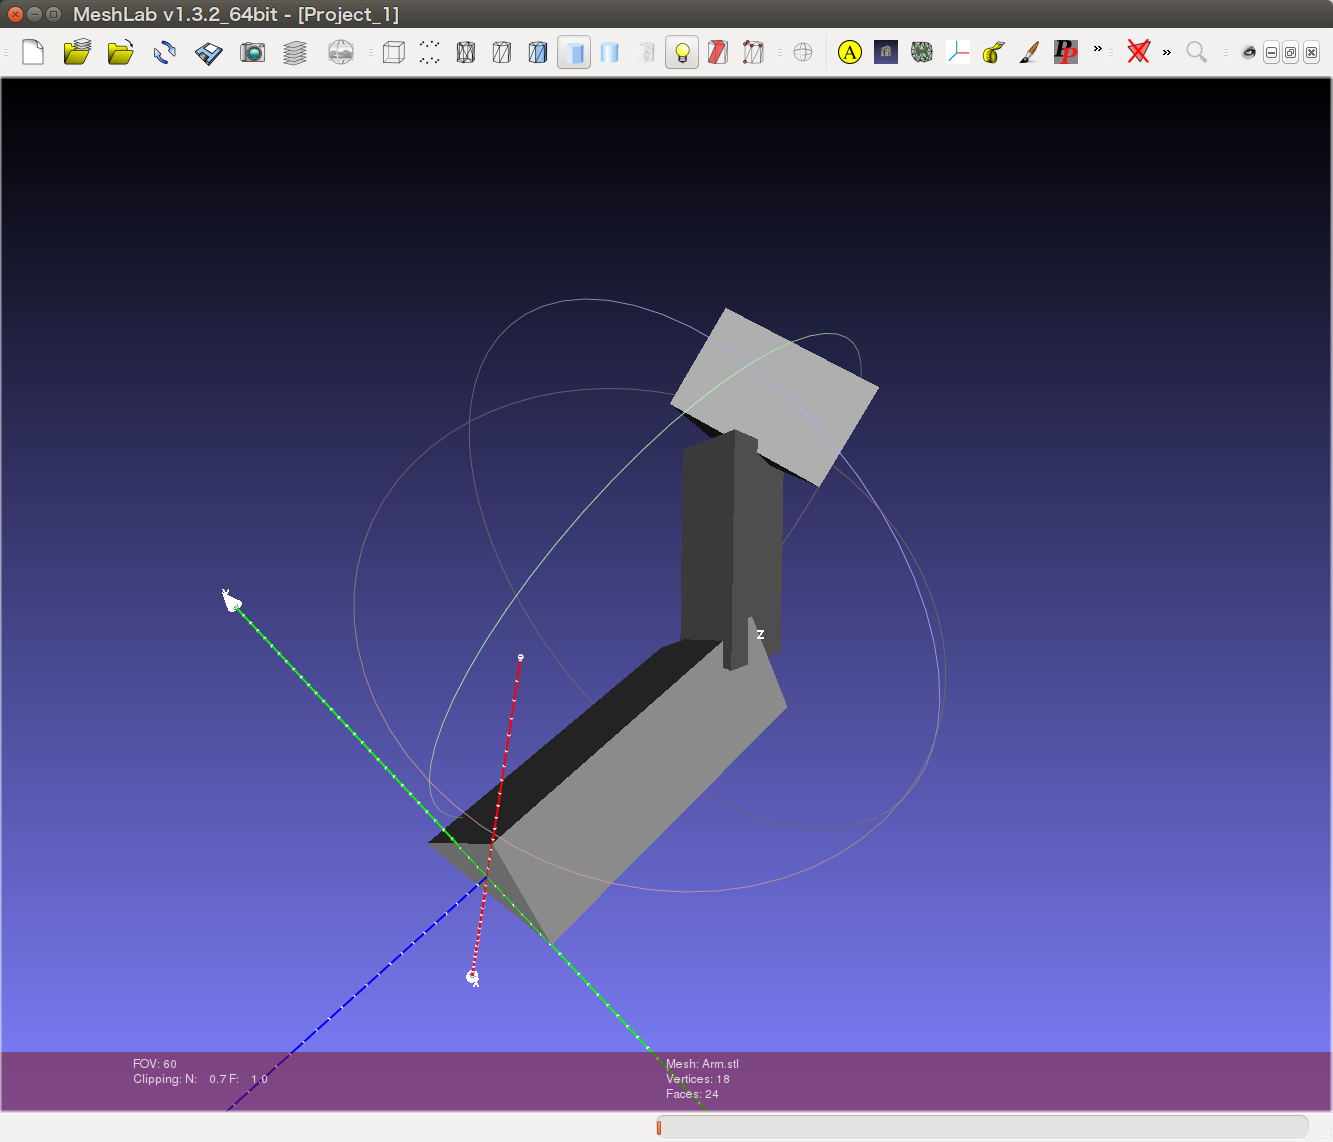
\includegraphics[width=70mm, bb = 0 0 1333 1142]{fig/png/arm4.png}
  \end{center}
  \caption{ロボットアームの姿勢4}
  \label{fig:ロボットアームの姿勢4}
 \end{minipage}
\end{figure}

\end{document}